\chapter{Lec 14 - Representation Learning}
\section{Representation Learning}
\textbf{Representation Learning} aims at learning representation of input data, typically by transforming it, such to make the input \textit{easier} for a classification or prediction task. The performance of any machine learning model is critically dependent on the representation used. The set of priors that should drive the choice of a representation is the following:
\begin{itemize}
    \item Smoothness
    \item Multiple explanatory factors
    \item A hierarchical organization of explanatory factors
    \item Sparsity
    \item ...
\end{itemize}

\section{Principal Component Analysis (PCA)}
Principal component analysis, or PCA, is a dimensionality-reduction method that is often used to reduce the dimensionality of large data sets, by transforming a large set of variables into a smaller one that still contains most of the information in the large set.\newline\newline
PCA tries to answer the following question: \textit{is there any other basis, which is a linear combination of the original one, that best re-express out data ?} In mathematical terms, PCA tries to re-express the dataset $\textbf{X} \in \mathbb{R}^{m \times n}$ (\textbf{examples on columns}) by a simple linear transformation $\textbf{P} \in \mathbb{R}^{m \times m}$:
\[\textbf{PX} = \hat{\textbf{X}}\]
Basically, we want to find the best transformation $\textbf{P}$ following some criteria.\newline\newline
The equation above is actually a change of basis that can be interpreted in different ways:
\begin{itemize}
    \item $\textbf{P}$ is a matrix that transforms $\textbf{X}$ into $\hat{\textbf{X}}$.

    \item Geometrically, $\textbf{P}$ transforms $\textbf{X}$ into $\hat{\textbf{X}}$ via a rotation and a stretching.

    \item The rows of $\textbf{P}$ are a new set of basis vectors.
\end{itemize}
Two phenomena can potentially \textit{contaminate} our data: \textbf{noise} and \textbf{redundancy}. The linear transformation we aim to find is the one that minimizes both the noise and the redundancy of the signal.\newline\newline
Both noise and redundancy can be estimated using measures related to the variance of the data:
\begin{itemize}
    \item The noise of a signal can be measured by the \textit{signal-to-noise} ratio (SNR):
    \[SNR = \frac{\sigma_{signal}}{\sigma_{noise}}\]

    \item Redundancy between features can be measured through their \textbf{covariance}, that is, how much are the features dependent by each other.
\end{itemize}
Given a dataset $\textbf{X} \in \mathbb{R}^{m \times n}$ (centered with mean 0) the \textbf{covariance matrix} $\textbf{S}_{\textbf{X}} \in \mathbb{R}^{m \times m}$ is computed as follows:
\[\textbf{S}_{\textbf{X}} = \frac{1}{n}\textbf{X}\textbf{X}^{T}\]
This matrix has as entries the covariances associated with all possible pairs of the initial features. Since the covariance of a variable with itself is its variance ($Cov(\textbf{X}_{i},\textbf{X}_{i})=Var(\textbf{X}_{i})$), in the main diagonal we actually have the variances of each initial feature. Furthermore, the covariance is commutative ($Cov(\textbf{X}_{i},\textbf{X}_{j})=Cov(\textbf{X}_{j},\textbf{X}_{i})$), so the entries of the covariance matrix are symmetric with respect to the main diagonal.\newline\newline
In order to reduce the features covariance, we want to have all the entries $\textbf{S}_{\textbf{X}}(i, j)$ equal to 0. So, the idea is to transform our data in a new representation $\hat{\textbf{X}}$ such that if we compute the covariance matrix of $\hat{\textbf{X}}$, we obtain a \textbf{diagonal matrix}.\newline\newline
In mathematical terms, the goal of PCA is to find some orthonormal matrix $\textbf{P}$ where $\hat{\textbf{X}} = \textbf{PX}$ such that
\[\textbf{S}_{\hat{\textbf{X}}} = \frac{1}{n}\hat{\textbf{X}}\hat{\textbf{X}}^{T}\]
is a diagonal matrix. \newline
The rows of $\textbf{P}$ are called \textbf{principal components}.\newline\newline
The PCA algorithm steps are:\newline
Given a dataset $\textbf{X} \in \mathbb{R}^{m \times n}$ (examples on the columns).
\begin{enumerate}
    \item Standardize the data. Center $\textbf{X}$ by subtracting off the mean of each measurement type.

    \item Compute the covariance matrix.

    \item Compute the \textbf{eigenvalues} ($\textbf{D} \in \mathbb{R}^{m \times m}$) and \textbf{eigenvectors} ($\textbf{E} \in \mathbb{R}^{m \times m}$) of the covariance matrix and set $\textbf{P} = \textbf{E}^{T}$.

    \item Select the $k << m$ most important component from $\textbf{P}$.
\end{enumerate}
Note that in step 4 is performed the dimensionality reduction. In fact, often the most interesting dynamics occur only in the first $k$ dimensions. Throwing out the less important axes can help to reveal hidden and simplified dynamics in high dimensional data.\newline\newline
Formally, given $k << m$, the dimensionality of $\textbf{X}$ is reduced by:
\[\textbf{P}_{k}\textbf{X} = \textbf{X}_{k} \in \mathbb{R}^{k \times n}\]
where $\textbf{P}_{k}$ is a sub-matrix of $\textbf{P}$ containing the $k$ most important component.\newline\newline
Interestingly, $\textbf{P}_{k}$ is also the minimizer of the squared \textbf{reconstruction error}:
\[min_{\textbf{P} \in \mathbb{R}^{k \times n}} ||\textbf{X} - \textbf{P}^{T}\textbf{P}\textbf{X}||^{2}_{F} \quad s.t. \,\, \textbf{P}\textbf{P}^{T} = \textbf{I}_{k \times k}\]
It represents how much is the loss in the transformation. This is because we obtain $\hat{\textbf{X}}$ by applying $\textbf{P}_{k}$ to $\textbf{X}$. So, applying $\textbf{P}_{k}^{T}$ to $\hat{\textbf{X}}$ is like \textit{going back} to $\textbf{X}$. However, if $k << m$ i don't obtain $\textbf{X}$ but something similar.

\subsection{Kernel PCA}
Kernel PCA extends the conventional PCA to deal with non-linear correlations using the \textbf{kernel trick}. A high level algorithm can be the following:
\begin{enumerate}
    \item Instead of using data points $\textbf{X}$ directly, we first map them to some feature space (implicitly).

    \item Center the data in the feature space.

    \item Implicitly extract principal components in the feature space, that is, apply PCA in the feature space. Projections of these principal components can be computed in terms of kernels only.

    \item The result will be non-linear transformations in the original input space.
\end{enumerate}

\subsection{PCA - Applications}
Some of the possible scenarios in which PCA can be useful:
\begin{itemize}
    \item Apply \textit{lossy compression}.
    \item Visualize the multi-dimensional data in 2D or 3D.
    \item Reduce the number of dimensions or discard noisy features.
    \item Perform a change of representation in order to make analysis of data at hand.
\end{itemize}

\section{Autoencoders}
Autoencoders (AEs) are an \textbf{unsupervised learning} technique based on feed forward neural networks. The aim of autoencoders is to learn a representation (often called \textit{encoding} or \textit{code}) for a set of data, typically for the purpose of dimensionality reduction. The network is composed by the following elements:
\begin{itemize}
    \item \textbf{Encoder:} Creates a new representation (the code) of the input
    \item \textbf{Decoder:} Reconstructs the input starting from the code
    \item \textbf{Bottleneck layer:} Hidden layer with a smaller dimensionality than the input layer (it makes the task harder). 
\end{itemize}
The goal of an autoencoder network is to \textit{copy} the input on its output. Basically, when we present an input example to the network, we want to obtain the same values in the output layer.
\begin{center}
    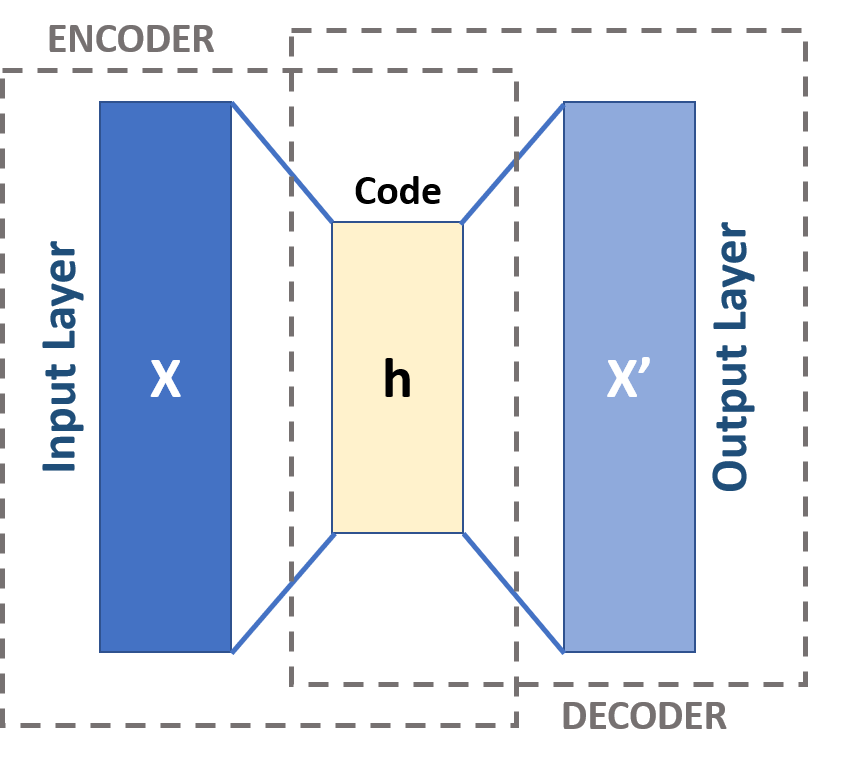
\includegraphics[scale = 0.4]{images/Autoencoder.png}
\end{center}
The easiest form of autencoder has:
\begin{itemize}
    \item A single hidden layer
    \item A set of parameters $\textbf{W}$, $\textbf{W}^{'}$ defined by two weight matrices and two bias vectors:
    \[\textbf{h} = f_{\textbf{W}}(\textbf{x}) = s_{1}(\textbf{Wx} + \textbf{b})\]
    \[\hat{\textbf{x}}= g_{\textbf{W}^{'}}(\textbf{h}) = s_{2}(\textbf{W}^{'}\textbf{h} + \textbf{b})\]
    where $s_{1}$ and $s_{2}$ denote the activation functions (for the hidden layer and the output layer respectively), which are usually non-linear.
\end{itemize}
The goal is to find the parameters $\textbf{W}$ and $\textbf{W}^{'}$ such that the output of the network approximates the input:
\[g_{\textbf{W}^{'}}(f_{\textbf{W}}(\textbf{x})) \approx \textbf{x}\]
The output of the hidden layer is a \textbf{new lower-dimensional representation} of the input.\newline\newline
The standard loss function is a mean squared error loss (called \textbf{reconstruction loss}):
\[L(\textbf{x}, \Tilde{\textbf{x}}) = ||\textbf{x} - \Tilde{\textbf{x}}||^{2}_{2}\]
where $\Tilde{\textbf{x}} = g_{\textbf{W}^{'}}(f_{\textbf{W}}(\textbf{x}))$. The final objective function that autoencoders aim to optimize is:
\[J(\textbf{W}, \textbf{W}^{'}; \textbf{X}) = \sum_{\textbf{x} \in \textbf{X}}L(\textbf{x}, g_{\textbf{W}^{'}}(f_{\textbf{W}}(\textbf{x})))\]
The learning procedure is performed using standard techniques for training neural networks, such as Backpropagation and Stochastic Gradient Descent.\newline\newline
A simple extension of autoencoders are Deep (non-linear) autoencoders:
\begin{itemize}
    \item \textbf{Deep AEs} add more hidden layers between the input and the code (as well as between the code and the output)
    \item \textbf{Non-linear AEs} set non-linear activation functions to the neurons.
\end{itemize}

\subsection{Regularized autoencoders}
Encodings produced by basic AEs do not generally present any special property. Additionally, like many other machine learning techniques, AEs are susceptible to overfitting. One possible technique to overcome these problems is to regularize the autoencoders.\newline\newline
\textbf{Regularized autoencoders} use a loss function that encourages the model to have other properties besides the ability to copy its input to its output:
\begin{itemize}
    \item \textbf{Sparsity} of the representation (most values for a given sample are zero or closed to zero)
    \item \textbf{Robustness} to noise or to missing inputs
    \item \textbf{Smallness} of the derivative of the representation
\end{itemize}
The general form of a regularized AE objective function is:
\[J(\Theta, \Theta^{'}; \textbf{X}) = \sum_{\textbf{x} \in \textbf{X}}L(\textbf{x}, g_{\Theta^{'}}(f_{\Theta}(\textbf{x}))) + \Omega(\Theta, \Theta^{'}; \textbf{X})\]
Basically, we want to find a trade-off between optimizing the reconstruction of the input and regularize the parameters.

\subsection{Denoising autoencoders}
The goal of Denoising autoencoders (DAE) is to clean the corrupted input. They have the same architecture of \textit{standard} autoencoders, but they are trained in a different way. The training process of a DAE works as follows:
\begin{itemize}
    \item The input \textbf{x} is corrupted into $\textbf{x}^{'}$ through a stochastic mapping: $\textbf{x}^{'} \sim q(\textbf{x}^{'} | \textbf{x})$.

    \item $\textbf{x}^{'}$ is then mapped to a hidden representation $\textbf{h} = f_{\Theta}(\textbf{x}^{'})$.

    \item Finally, the model reconstructs the input.
\end{itemize}

\section{Convolutional Neural Networks (CNN)}
Convolutional Neural Networks are a specialized kind of NN for processing data that has a \textbf{grid-like topology} (e.g. images). The name CNN indicates that the network employs a mathematical operation called \textbf{convolution}.\newline\newline
CNN learns different levels of abstraction of the input, e.g. for images:
\begin{itemize}
    \item in the first few hidden layers, the CNN usually detects general pattern, like edges.

    \item the deeper we go into the CNN, these learned abstractions become more specific, like textures, patterns and parts of objects.

\end{itemize}

\subsection{Convolution}
Let's say that we have an image as input. Convolution is a mathematical operation that works by moving a sliding window (kernel) through the image, pixel by pixel. The window contains coefficients which characterize the transformation. At each position, the result of the convolution is calculated by combining the values of the image subtended to the window with the coefficients of the window itself. In order to compute the new value of the central pixel, the coefficients are:
\begin{enumerate}
    \item multiplied by the values of the original image subtended to the window
    \item added
\end{enumerate}
\textbf{Borders:}\newline
Given an $n \times n$ kernel, its external row/column coincides with the border of the image when the center of this mask is at distance $\frac{n-1}{2}$ from the edge. If you move further out, part of the window \textit{leaves} the image.\newline
This situation can be managed in three different ways:
\begin{itemize}
    \item limit the movement of the mask, keeping it at a minimum distance of $\frac{n-1}{2}$ from the edges.
    \item duplicate the external rows/columns of the image
    \item enlarge the image with rows/columns of zeros
\end{itemize}
Solution 1 gives reliable results, but produces a different size image from the original. Solutions 2 and 3, on the other hand, give results that are not exactly authentic near the edges, but are often convenient because they allow you to obtain an output image with the same size as the input one.\newline\newline
For what concerning convolution of multi-channel images, we perform the convolution for each channel and we sum up the results.
\begin{center}
    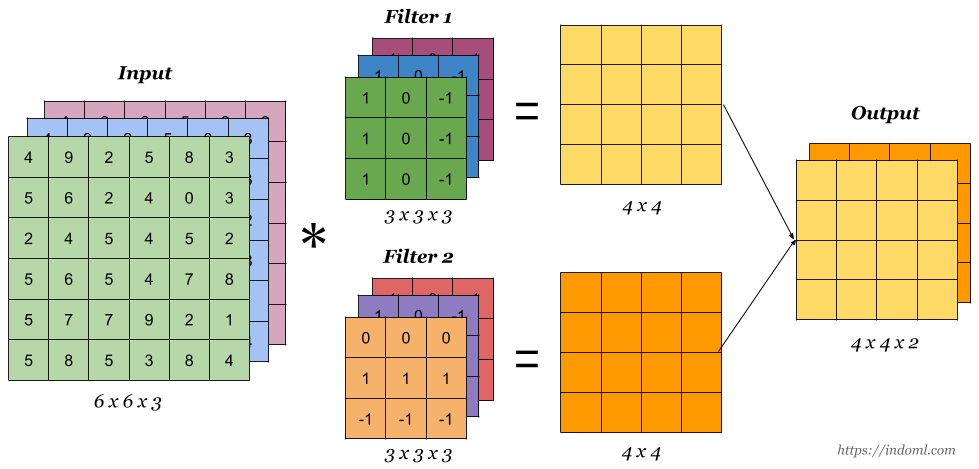
\includegraphics[scale = 0.3]{images/Convolution.png}
\end{center}
Note that if we apply $k$ filters, the output will be a tensor with $(n \times m \times k)$ dimension. 

\subsection{Pooling}
Another commonly used technique in CNN is \textbf{Pooling}.\newline\newline
Pooling layer is used to reduce the size of the representations and to speed up calculations, as well as to make some features it detects a bit more robust.
\begin{itemize}
    \item \textbf{Max pooling:} It gets the maximum value of the pixels for each section of the image.

    \item \textbf{Average pooling:} It gets the average value of the pixels for each section of the image.
\end{itemize}
\begin{center}
    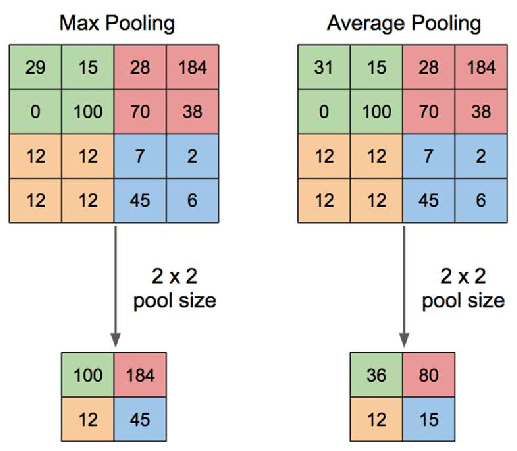
\includegraphics[scale = 0.3]{images/pooling.png}
\end{center}

\subsection{Convolution layer}
The Convolution layer applies a set of filters to the input data (performing convolution) in order to extract features or representations from the data. The result is usually passed through an activation function (ReLu) in order to achieve non linearity. \newline\newline
Basically, a CNN is a sequence of convolution layers and sub-sampling layers with a fully-connected layer at the end.
\begin{center}
    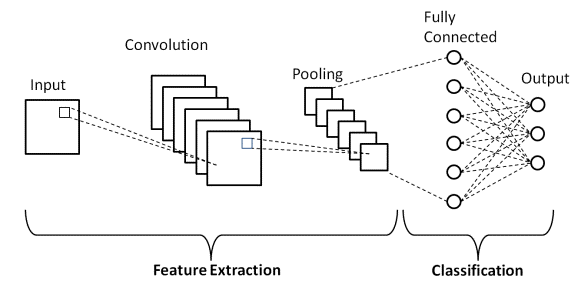
\includegraphics[scale = 0.7]{images/CNN.png}
\end{center}

\section{Word Embedding - Word2Vec}
(Neural) \textbf{Word embedding} belongs to the text pre-processing phase. The goal is to transform a text (set of words) into a vector of numbers such that similar words produce similar vectors. The word2vec technique is based on a feed-forward, fully connected architecture. It is similar to an autoencoder, but rather than performing input reconstruction, word2vec trains words according to other words that are neighbors in the input corpus (called \textbf{context}).\newline\newline
Word2vec aims at computing a \textbf{vector} representation of words able to capture semantic and syntactic word similarity.\newline\newline
By using this concept of context, word2vec can learn word embedding in two different ways:
\begin{itemize}
    \item \textbf{CBOW} (Continuous Bag of Words) in which the neural network uses the context to predict a target word.

    \item \textbf{Skip-gram} in which it uses the target word to predict a target context.
\end{itemize}
\begin{center}
    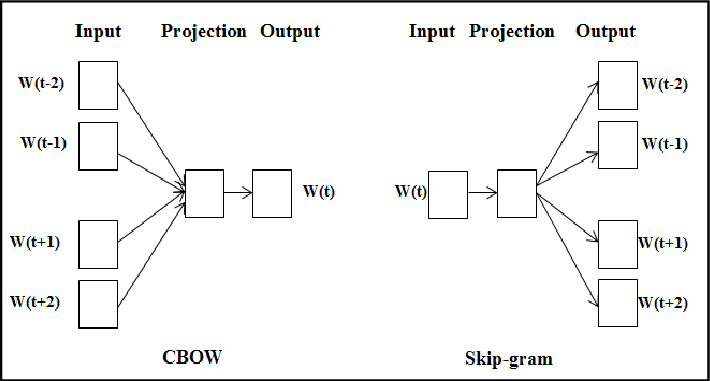
\includegraphics[scale = 0.3]{images/word2vec.png}
\end{center}
\subsection{Word2Vec Skip-gram model}
The input of the model is the one-hot encoding of the word according to a vocabulary.
The output is a distribution over the words of being in the context of the target word. The formal method is defined as follows:
\[\textbf{h} = \textbf{W}^{T}\textbf{x}\]
\[\textbf{u} = \textbf{W}^{'T}\textbf{h} = \textbf{W}^{'T}\textbf{W}^{T}\textbf{x}\]
\[\textbf{y} = \sigma(\textbf{u})\]
where $\sigma(\cdot)$ is the \textbf{softmax} function.\newline\newline
The goal of skip-gram model is to maximize the \textbf{average log probability}.
\begin{center}
    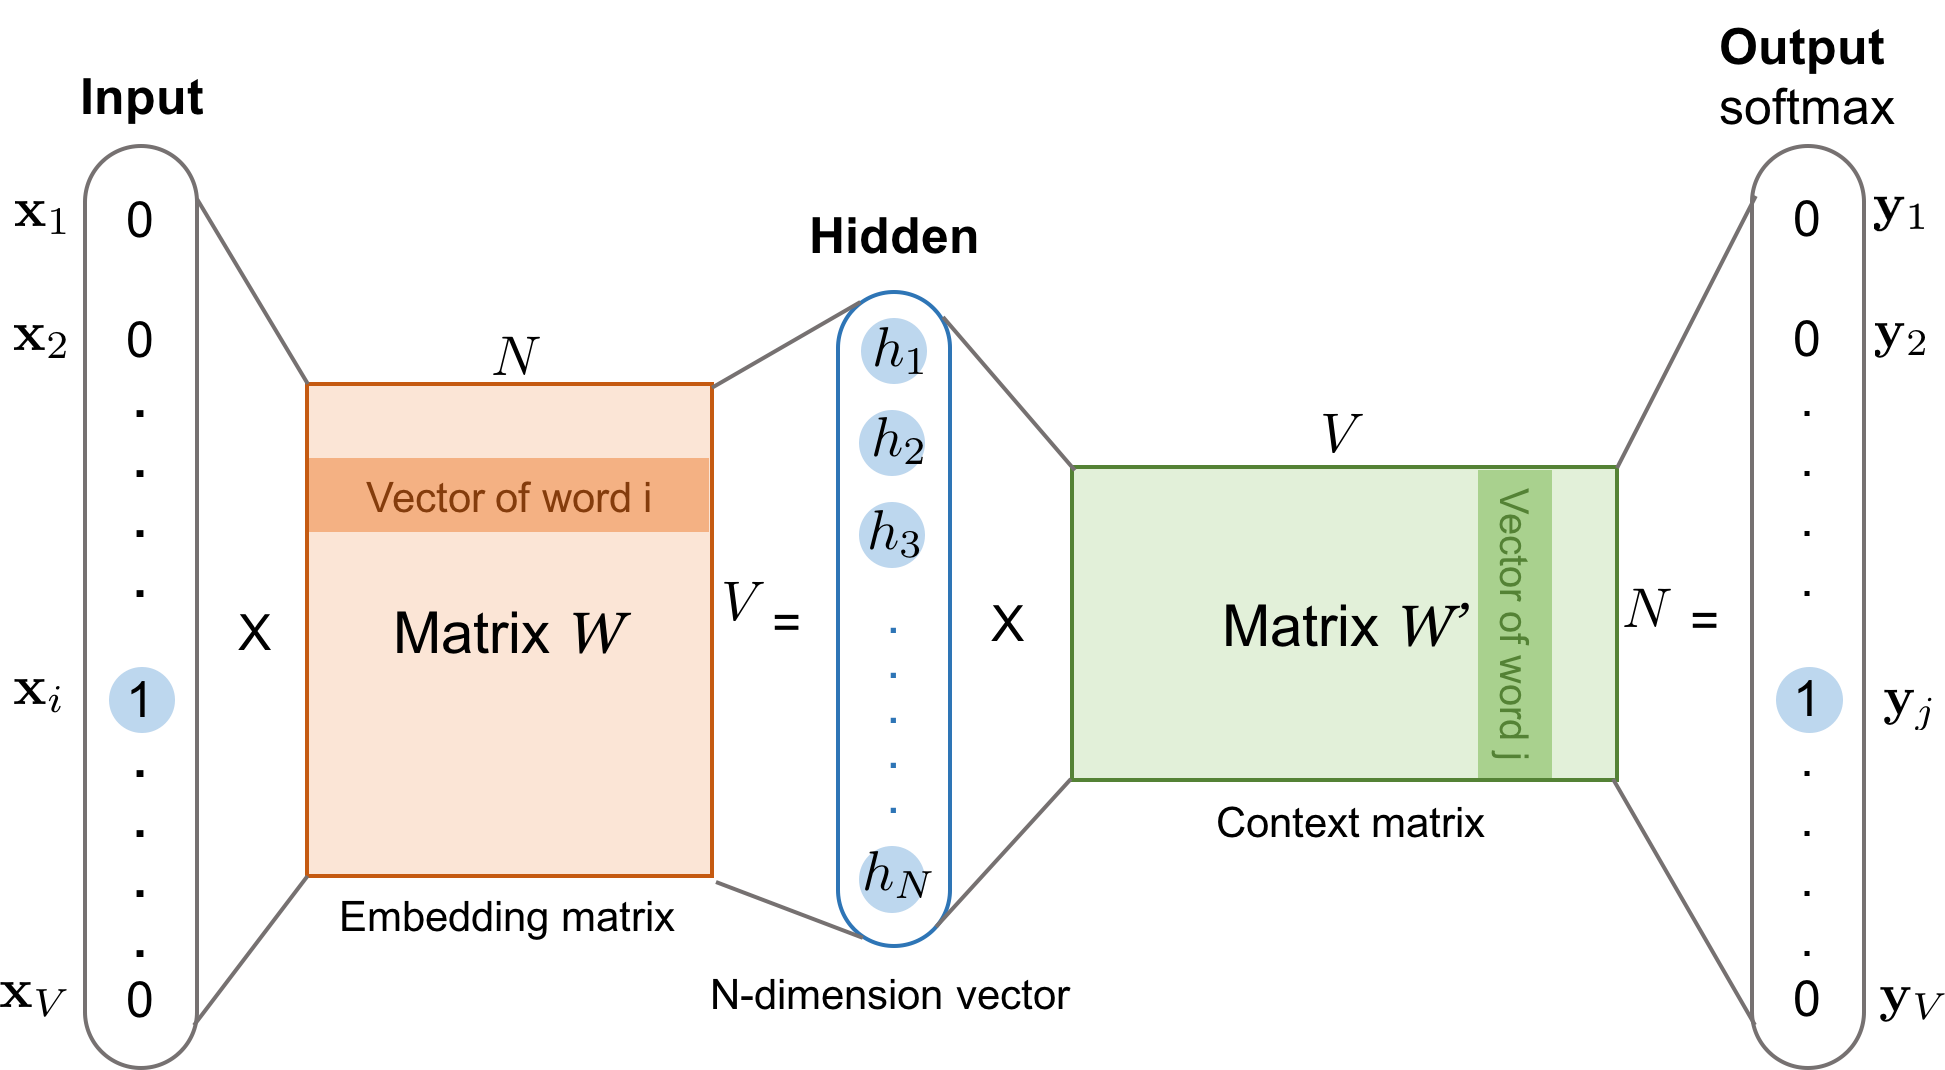
\includegraphics[scale = 0.3]{images/skip-gram.png}
\end{center}

\subsection{Word2Vec - Semantic and syntactic relations}
Word2vec captures different degrees of similarity between words. For example, patterns such as \textit{Man is to Woman as Brother is to Sister} can be generated through algebraic operations on the vectors representations of the words.
\[Brother - Man + Woman \approx Sister\]

\section{Knowledge graph}
A knowledge graph (KG) is a multi-relational graph composed of entities (nodes) and relations (edges). Edges are represented as triples of the form \textit{(head entity, relation, tail entity)} also called \textbf{facts}, indicating that two entities are connected by a specific relation.\newline\newline
Formally, given a KG of facts $S$, a relation is denoted by a triple $(h, r, t) \in S$ where:
\begin{itemize}
    \item $h$ is the \textbf{head} of the relation
    \item $r$ is the kind of relation
    \item $t$ is the \textbf{tail} of the relation
\end{itemize}
We assume that $h, t \in \epsilon$ where $\epsilon$ is the set of all possible entities and $r \in R$ where $R$ is the set of all possible relations. 

\subsection{Trans-E}
The basic idea behind Trans-E is that a relation corresponds to a linear translation in the embedding space. The method assumes that entities can be mapped into a $k$-dimensional embedding space ($h,t \rightarrow \textbf{h},\textbf{t} \in \mathbb{R}^{k}$) in which when the relation $(h, r, t)$ holds, then $\textbf{h} + \textbf{r} \approx \textbf{t}$. Otherwise, $\textbf{t}$ should be far away from $\textbf{h} + \textbf{r}$.

